\scanpage{241}

du cor 1 précédent, et le système des $\underline{\operatorname{Pic}}_{X_{\unsure{n|0}}/k}(k)$ satisfait à M.L.

\margin{\figure{\begin{tikzpicture}
\node[draw,ellipse,rotate=25,align=left,inner sep=8pt] {\uline{N.B.} les\\\unsure{grs} $=$ \unsure{vérifient}\\M.L.A.R.};
\end{tikzpicture}}}

\uline{N.B.} On suppose l'existence des $\underline{\operatorname{Pic}}_{X_n/k}$. Elle est prouvée en général par \uline{Murre}. Dans le cas projectif, on le sait par Grothendieck -- Oort.

Le fait que les $\underline{\operatorname{Pic}}_{X_{n+1}/k}\longrightarrow\underline{\operatorname{Pic}}_{X_n/k}$ sont de type fini, \deleted{et} les noyaux \deleted{sans torsion} unipotents, les conoyaux sans torsion, se voit par la \unsure{théorie|thèse} de Oort \deleted{\unsure{et}} \deleted{des obstructions} [cf suite ex. de cohomologie]. De plus, on utilise le th. \inserted{\figure{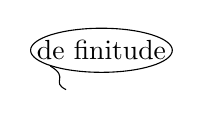
\begin{tikzpicture}[baseline=-.5ex]\draw (0,0) ellipse (.9 and .28);\node at (0,0) {de finitude};\draw (-.65,-.2)..controls(-.4,-.35)and(-.65,-.4)..(-.45,-.5);\end{tikzpicture}}} de Néron \deleted{\unsure{Séveri}} pour $\underline{\operatorname{Pic}}_{X_0/k}$.

\margin{\figure{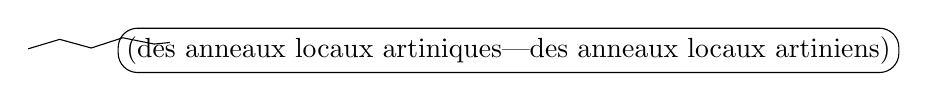
\begin{tikzpicture}\node[draw,rounded corners=7pt,inner sep=3pt] at (0,0) {(\unsure{des anneaux locaux artiniques|des anneaux locaux artiniens})};\draw (-4.3,.1)--(-4.5,.08)--(-4.9,.16)--(-5.3,.03)--(-5.7,.14)--(-6.1,.02);\end{tikzpicture}}}
\margin{\figure{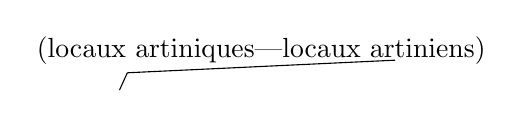
\begin{tikzpicture}\node at (0,0) {(\unsure{locaux artiniques|locaux artiniens})};\draw (-1.7,-.28)--(1.7,-.12);\draw (-1.7,-.28)--(-1.8,-.5);\end{tikzpicture}}}

\uline{Corollaire} \inserted{Soit $\mathfrak X$ préschém. \unsure{formel} propre sur un anneau local noeth. complet à corps résiduel $k$ de car. 0. Supposons que les comp. connexes de $X_0$ soient géomt. connexes et \unsure{admettent un pt rat/$k$}. Alors} le système projectif $(\operatorname{Pic}(X_n))_{n\in\unsure{\mathbf Z|\mathbf N}}$ satisfait à M.L.

\figure{\begin{tikzpicture}[x=1cm,y=1cm]
\draw (0,0) -- (0,1.1);
\end{tikzpicture}}

\margin{On \unsure{peut} supposer $k\subset A$ \unsure{grâce à Cohen}.}

\deleted{Lorsque les composantes connexes de $X_0$ sont géomt. connexes, et que \unsure{ces dernières} \unsure{admettent} un pt rat/$k$, cela \unsure{provient du}}
\inserted{\unsure{provient de}}

\mspage{240}
